% ##################################################################################################################
\section{Munich}
\label{sec:munich}
\hfill \textbf{Author:} Benjamin Kickhöfer

\editdone{This text has undergone the professional edit. Please no grammatical changes anymore! They are most-probably wrong.}

% ##################################################################################################################
The \gls{matsim} scenario for the Munich metropolitan area was set up during 2010.%
%
\footnote{
%
Detailed descriptions of the scenario can be found in \citet{KickhoeferEtAl_VanoutriveVerhetsel_2013} and \citet{Kickhoefer_PhDThesis_2014}.
%
}
%
The main goal was, and is, simulation of local air pollutant and global greenhouse gas emissions and how their levels change with different policy measures---on aggregated and spatially disaggregated levels. Thus the scenario was used for development and testing of the \gls{emt} (see Chapter~\ref{ch:emissions}). For an example illustrating where overall $\mathit{NO_2}$ private car and freight vehicle emissions are produced over one day, see Figure~\ref{fig:munich:no2emissions}.
%
\createfigure%
{$\mathit{NO_2}$ emissions in Munich}%
{$\mathit{NO_2}$ emissions in Munich}%
{\label{fig:munich:no2emissions}}%
{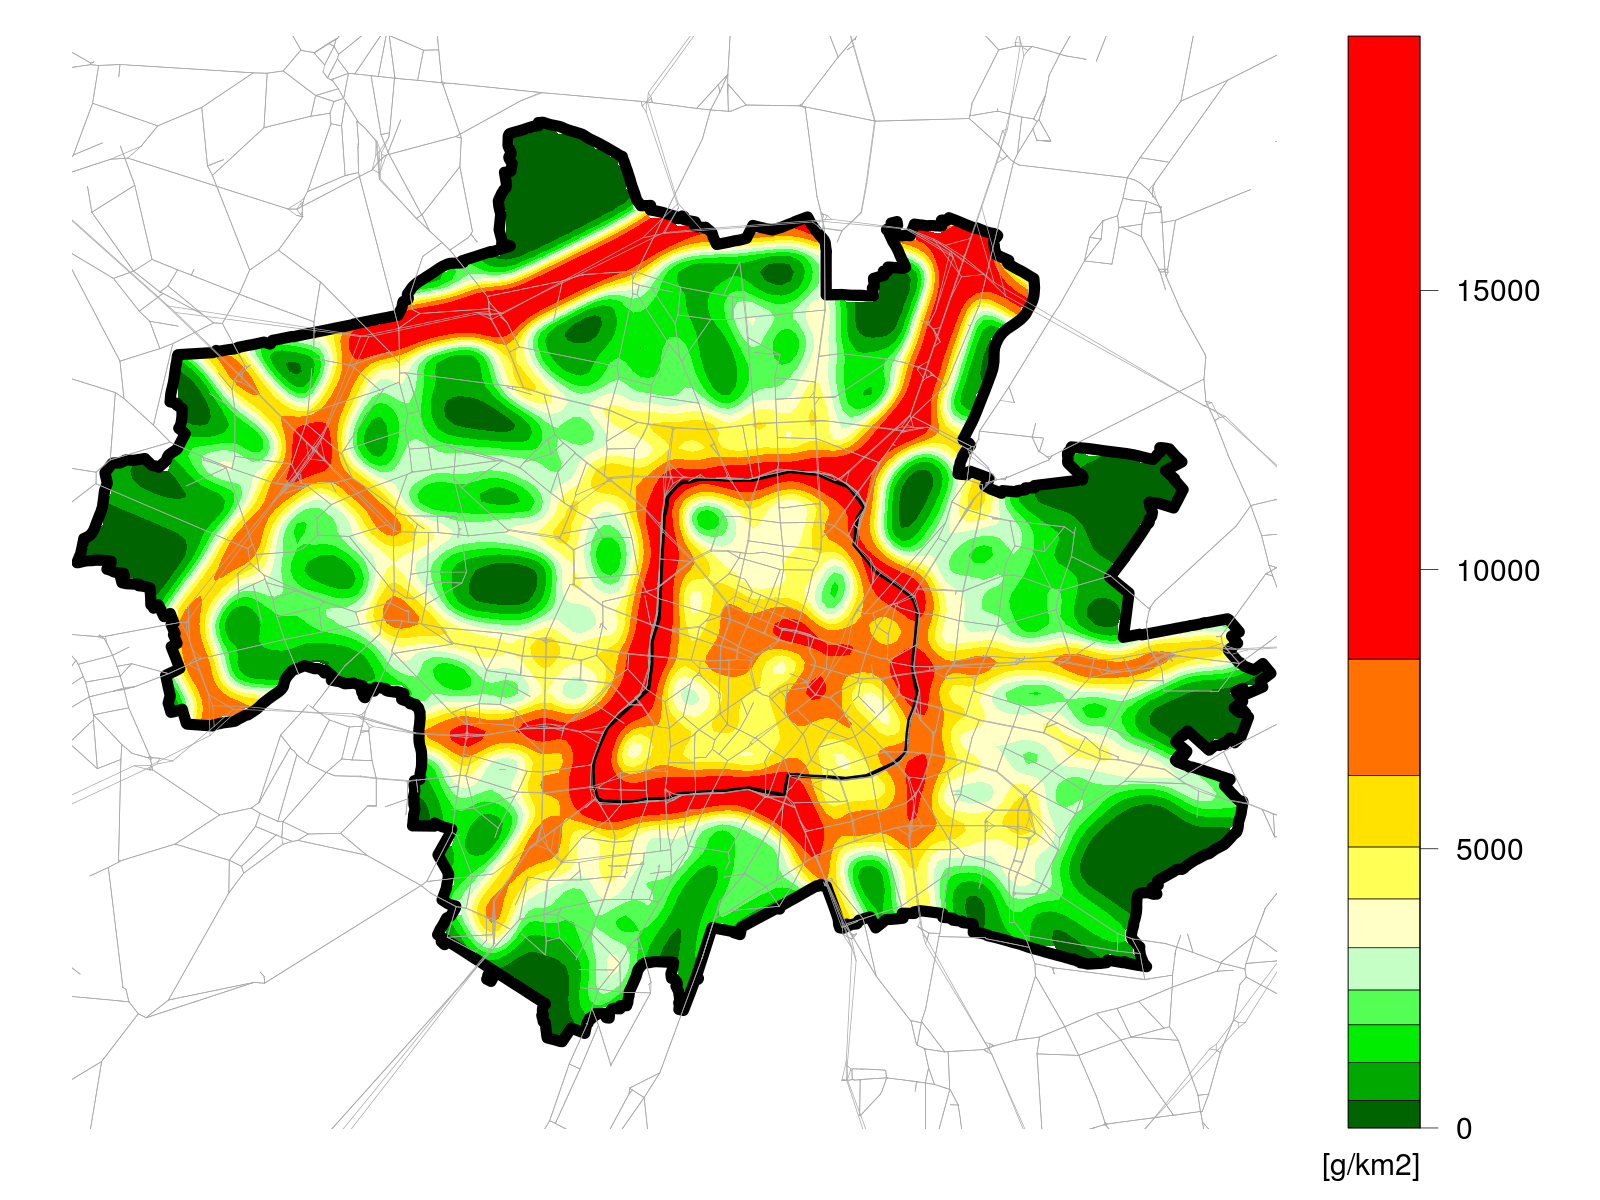
\includegraphics[width=0.85\textwidth, angle=0]{./using/figures/baseCase_1500_NO2_g_108000_0.png}}%
{}

Network information from \acrshort{visum} was converted into \gls{matsim} format, resulting in a network of 17\,888 nodes and 41\,942 links.
%
This transport supply was then linked to travel demand from different sources; an inner-urban traffic activity-based demand from survey data was created, based on \gls{mid} \citep[MiD 2002,][]{FollmerEtAl_TechRep_infasDIW_2004}. This synthetic population segment consisted of roughly 1.4\,million individuals, with detailed vehicle information for every household.
%
Commuters and reverse commuters were modeled with data provided by the German Federal Employment Office \citep{BoehmeEigenhueller_TechRep_IAB_2006}. This part of the population consisted of approximately 0.5\,million individuals, with  0.3\,million commuting to Munich for work. The rest lived in Munich and commuted to their workplace around the city.
%
Freight traffic was also introduced into the model using data from the German Ministry for Transport \citep{ITBBVU_TechRep_2007}. This group consisted of roughly 0.15\,million freight vehicles, performing one commercial trip per day.

The scenario was used for several case studies:
%
\citet{HuelsmannEtAl_LAS_2011} used a single street corridor to validate simulated travel times and emission levels against actual data obtained from a test vehicle.
%
\citet{KickhoeferEtAl_VanoutriveVerhetsel_2013} investigated the relationship between the price elasticities of car travel demand and air pollutant emissions.
%
\citet{HuelsmannEtAl_GerikeEtAl_2013} identified city areas with high air pollution concentration. They defined these areas as "hotspots", exceedomg the \gls{eu} limits for \gls{no2}. The authors raised toll levels incrementally for vehicles passing these hotspots, until high pollution concentrations disappeared, to estimate true threshold value \gls{eu} avoidance costs.
%
\citet{KickhoeferNagel2012EmissionInternalization} derived time-dependent, vehicle-specific, first-best air pollution tolls to create a benchmark for real-world policy evaluation.
%
\citet{KickhoeferKern_MobilTUM_2014} went one step further and calculated time-dependent, vehicle-specific air pollution exposure tolls to correct toll levels with \citet{KickhoeferNagel2012EmissionInternalization} for a count of individuals affected.



% ##################################################################################################################